 
 %\setcounter{page}{45}
 \clearpage
 %\pagenumbering{arabic}
 \newpage
 % \addcontentsline{toc}{chapter}{\hfill 34}
 \addtocontents{toc}{\protect\contentsline{chapter}{CAPÍTULO IV. Propuesta de diseño   \hfill  110}{}{}}
 
 

 \begin{titlepage}
 	
 	
 	\centering
 	\begin{tikzpicture}%opacity=0.5
 		\node[inner sep=0pt, ] (image) at (0,0) {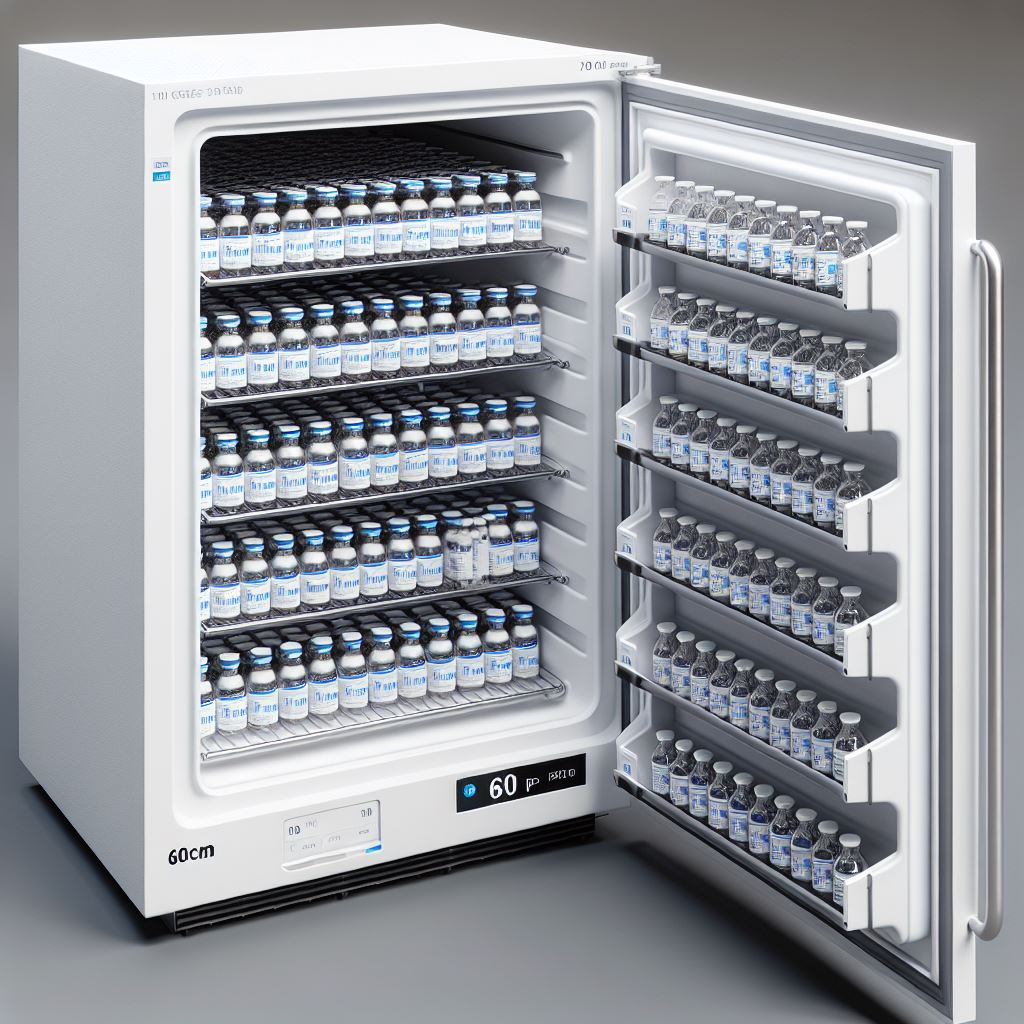
\includegraphics[width=\textwidth]{figures/FinalDesigner}};
 		\fill [white,path fading=south] (-5,-4) rectangle (5,4);
 		\node[black,font=\Huge\bfseries] at (0,3) {Capítulo V. Análisis de costos del proyecto};
 		\node[black,font=\Large\bfseries] at (0,1) {Estudio de costos del proyecto};
 		\node[black,font=\Large\bfseries] at (0,0) {Costos directos};
 			\node[black,font=\Large\bfseries] at (0,-1) {Costos indirectos};
 		\node[black,font=\Large\bfseries] at (0,-2) {Estimación del costo del proyecto};
 	\end{tikzpicture}
 \end{titlepage}
 
 \newpage 
 
 \section*{Introducción}
 
 
 

 \setcounter{chapter}{5}
 \setcounter{page}{111}   
 \setcounter{section}{0}
 \setcounter{figure}{0}
 \setcounter{table}{0}
  \addcontentsline{toc}{section}{{Introducción}} 
La distribución de la cámara de refrigeración se detalla en la Figura \ref{fig:4-propuestasol}. El contenedor del refrigerador está adaptado con láminas compuestas de poliuretano (película interna $f_i$ - Poliuretano - película externa $f_e$) en las cuatro paredes, con el objetivo de minimizar la pérdida de temperatura por transferencia térmica a través de las superficies. Esta aislación contribuye a evitar el uso de ventiladores, mejorando la eficiencia energética en las etapas iniciales del funcionamiento.

En la parte posterior de la cámara se integra la unidad de refrigeración, cuya función es proteger los componentes del sistema. Esta unidad alberga los elementos principales, como el compresor, el condensador y el dispositivo de expansión, que están conectados directamente al evaporador. El evaporador está situado en el interior de la cámara y conectado al serpentín, cuya función es asegurar una mejor distribución del refrigerante dentro de la cámara, lo que permite una disipación de calor más eficiente y uniforme.

Además, la cámara está equipada con diversas tapas y una cubierta de cristal, diseñadas para mantener el medicamento en condiciones óptimas de almacenamiento.

La cámara tiene dimensiones de 60 × 60 × 51.2 centímetros. Es fundamental considerar aspectos como el flujo de aire interno y la distribución térmica. La selección del serpentín garantizará una transferencia de calor eficiente y uniforme, minimizando las zonas frías o calientes que podrían afectar la integridad del producto. Además, en los cálculos de secciones posteriores se considera la capacidad del evaporador para manejar la carga térmica en función de la cantidad y tipo de insulina almacenada, así como las condiciones ambientales externas propias de la Alcaldía.

 \section{Costos Directos}
 Son aquellos costos que tienen una conexión directa con el proyecto y se reflejan de manera tangible; se manifiestan en el desarrollo del proyecto y en la conclusión de este. Son los costos responsables de manifestar de manera tangible aquello que en su principio fue una propuesta de solución, tanto en los componentes de la obra, como en los operadores responsables del desarrollo del proyecto.
 
 \subsection{Mano de obra}
 Para el desarrollo del proyecto se necesita de apoyo técnico y personal capacitado para la ejecución e instalación de componentes específicos. En este proyecto, es fundamental contar con técnicos especializados para la instalación de la unidad de refrigeración, cuyo sistema garantizará la correcta refrigeración del medicamento en cuestión, y debe estar adaptado a las necesidades específicas del entorno de almacenamiento.
 
 
 Según las tarifas estimadas por el Gobierno de México y la Secretaría de Economía del México, los técnicos especializados en instalación de sistemas de refrigeración tienen un salario aproximado de \$10,250.00 MXN por instalación. Este cálculo proviene de fuentes especializadas en la instalación y puesta en marcha de sistemas de refrigeración, y se estima que el tiempo necesario para la instalación de todos los componentes, incluidos los trabajos de aislamiento, es de aproximadamente 2,400 minutos, lo que equivale a un tiempo máximo de trabajo de 5 días.

 \subsection{Distribución y Características de la Cámara de Refrigeración}
 \subsection{Consideraciones del Producto}
Las dimensiones de la cámara son 60 × 60 × 51.2 centímetros, lo que permite una distribución eficiente del aire y una distribución térmica adecuada. En este sentido, la selección del serpentín será clave para garantizar una transferencia de calor eficiente y minimizar las zonas frías o calientes que podrían afectar la integridad del producto. Además, la capacidad del evaporador se seleccionará en función de la carga térmica generada por la cantidad y tipo de insulina almacenada, así como las condiciones ambientales externas propias de la Alcaldía de Azcapotzalco.


 \subsubsection{Unidad Condensadora}
 La selección de la unidad condensadora toma en cuenta los siguientes parámetros esenciales para el correcto funcionamiento del sistema de refrigeración en la cámara destinada al almacenamiento de insulina:
 
 \begin{itemize}
 	\item \textbf{Carga térmica:} 0.0882 T.R. = 1,058.6 BTU/h
 	\item \textbf{Temperatura de almacenamiento:} 3 °C (39.2 °F)
 	\item \textbf{Temperatura de evaporación del refrigerante:} -20 °C (-4 °F)
 	\item \textbf{Temperatura del exterior:} 25 °C (77 °F)
 	\item \textbf{Temperatura de condensación del refrigerante:} 33.5 °C (92.3 °F)
 \end{itemize}
 
 Además de estos parámetros, es necesario considerar el tipo de refrigerante que emplea la unidad, ya que es el fluido de trabajo con el que opera todo el sistema. Se opta por el uso del refrigerante R-134a debido a su adecuado desempeño para sistemas de refrigeración de baja capacidad y temperaturas moderadas, como las requeridas en tu diseño. Este refrigerante ofrece una excelente eficiencia energética, es químicamente estable, tiene un bajo potencial de agotamiento de la capa de ozono (ODP=0), y cumple con normativas internacionales para aplicaciones médicas y farmacéuticas. Además, su disponibilidad en el mercado mexicano y su compatibilidad con compresores de pequeña escala y sistemas compactos lo hacen una opción viable. Los criterios de selección incluyen la capacidad de transferencia térmica, compatibilidad con los materiales de construcción del sistema, seguridad (baja toxicidad e inflamabilidad), impacto ambiental (bajo GWP), y facilidad de mantenimiento. Estas características lo posicionan como una solución eficiente, segura y sostenible para tu cámara de refrigeración. Si tu diseño requiere temperaturas extremadamente bajas, también podría evaluarse el uso de R-404A, aunque este tiene un mayor impacto ambiental.

Además cabe señalar que se elige dicho refriqerante ya que es el que maneja la unidad evaporadora, lo que garantiza la compatibilidad y eficiencia en el sistema de refrigeración.
 
 Es importante destacar que la elección de la unidad condensadora y el refrigerante deben ser coherentes con las condiciones operativas de la cámara de refrigeración y la carga térmica que se manejará, para evitar fluctuaciones de temperatura que puedan comprometer la efectividad del almacenamiento del medicamento.
 

 La cámara de refrigeración se encuentra diseñada para mantener las condiciones óptimas para el almacenamiento de insulina. La distribución del espacio y los componentes de la cámara se detallan en la figura 4.1, destacando el uso de láminas compuestas de poliuretano para minimizar la pérdida de temperatura por transferencia térmica. Estas láminas están ubicadas en las cuatro paredes de la cámara, lo que contribuye a evitar el uso de ventiladores y mejora la eficiencia energética en las etapas iniciales del funcionamiento.
 
 
 En la parte posterior de la cámara, se integra la unidad de refrigeración, cuya función es proteger los componentes del sistema. Esta unidad alberga los elementos principales, como el compresor, el condensador y el dispositivo de expansión, los cuales están conectados directamente al evaporador. El evaporador está ubicado en el interior de la cámara y conectado al serpentín, que asegura una distribución adecuada del refrigerante dentro de la cámara, permitiendo una disipación de calor más eficiente y uniforme.
 

 
 \subsection{Comparación de Unidades Condensadoras}
 
 El análisis a continuación presenta las características y ventajas de las unidades condensadoras BOHN e Ice Shadow, comparando tres opciones disponibles para la refrigeración en la UMF40. La elección de la unidad adecuada dependerá de varios factores, como la carga térmica necesaria, el costo y la facilidad de mantenimiento.
 
% Please add the following required packages to your document preamble:
% \usepackage{booktabs}
% Please add the following required packages to your document preamble:
% \usepackage{booktabs}
% 
% Beamer presentation requires \usepackage{colortbl} instead of \usepackage[table,xcdraw]{xcolor}
\begin{table}[H]
	\caption{Comparación de unidades condensadoras de Temperatura BAJA}
	Fuente: Elaboración propia, basado de \cite{bohn}.
	\centering
	  \scalebox{0.7}{ 
\begin{tabular}{@{}ccllccl@{}}
	\cmidrule(r){1-6}
	\textbf{Opción}   & \textbf{Proveedor/Marca} & \multicolumn{1}{c}{\textbf{Ventajas}}                                                                                                                                                           & \multicolumn{1}{c}{\textbf{Desventajas}}                                                                                                                               & \textbf{Costo\footnote{Al la fecha 13/diciembre/2024 el dólar amerciano (USD) tiene un costo de \$20.16 MXN}} & \multicolumn{1}{l}{\textbf{Elección}} &   \\ \cmidrule(r){1-6}
	\begin{tabular}[c]{@{}c@{}}IMCON012\\ 1/8 HP\end{tabular} & ICE SHADOW               & \begin{tabular}[c]{@{}l@{}}- Cumple con la carga \\       térmica necesaria. \\ - Facilidad de mantenimiento. \\ - Supervisor de consumo \\       de combustible. \\ - Silencioso.\end{tabular} & \begin{tabular}[c]{@{}l@{}}- El deshielo eléctrico \\ aumenta la carga térmica.\end{tabular}                                                                           & \$90 USD       &\textbf{ \textcolor[HTML]{34ff34}{ \checkmark }} &  \\ \cmidrule(lr){3-4}
\begin{tabular}[c]{@{}c@{}}CH161L6B\\ 1/4 HP\end{tabular}         & BOHN                     & \begin{tabular}[c]{@{}l@{}}- Marca Líder en el mercad. \\ - Facilidad de mantenimiento.\\ - Carga térmica aproximada.\end{tabular}                                                              & \begin{tabular}[c]{@{}l@{}}- No cumple con la carga \\       térmica requerida. \\ - Costo elevado .\\ - Diseñado para equipos \\     un poco más grandes\end{tabular} & \$9,095.00  USD    & \textbf{\textcolor[HTML]{fd6864}{\text{x}}}    &   \\ \cmidrule(lr){3-4}
\begin{tabular}[c]{@{}c@{}}CH111L6 \\ 1/4HP\end{tabular}         & BOHN                     & \begin{tabular}[c]{@{}l@{}}- Marca Líder en el mercad. \\ - Facilidad de mantenimiento.\\ - Carga térmica cerca a la necesitada.\end{tabular}                                                   & \begin{tabular}[c]{@{}l@{}}- No cumple con la carga\\     térmica requerida. \\ - Costo elevado..\\ - Diseñado para equipos \\      un poco más grandes\end{tabular}   & \$7,750.00  USD    & \textbf{\textcolor[HTML]{fd6864}{\text{x}}}    &   \\ \cmidrule(r){1-6}
\end{tabular}
}
\end{table}
 
 \subsubsection{Análisis de las Opciones}
 Cada una de las opciones presenta características particulares que pueden ser relevantes dependiendo de las necesidades específicas del proyecto en la UMF40. Se debe considerar que el costo es un factor importante, pero también lo es la eficiencia en el mantenimiento y la capacidad de enfriamiento.
 
 \begin{itemize}
 	\item \textbf{IMCON012 1/8 HP} Es la opción que mejor cumple con la carga térmica necesaria para el almacenamiento de insulina en la UMF40. Destaca por su fácil mantenimiento y el control del consumo de combustible. Además de ser una marca comercial muy común dentro del país.
 	\item \textbf{CH161L6B 1/4HP} Aunque es silenciosa y de fácil uso, no cumple con los requerimientos de carga térmica. Su costo también es elevado en relación con su utilidad en este proyecto, añadiendo su funcionalidad sobrada para la cámara diseñada, lo que puede hacerla menos atractiva para este tipo de proyecto.
 	\item \textbf{CH111L6B 1/4HP} Ofrece un menor tiempo de desescarche y un precio más bajo, pero carece de la funcionalidad de seguimiento del consumo de combustible y de carga térmica, lo que podría ser un inconveniente en términos de eficiencia energética.
 \end{itemize}
 
 \subsubsection{Preferencia y Elección}
La elección final se ha basado en los principios de los requisitos específicos de la cámara de refrigeración, así como en el presupuesto público disponible para la unidad condensadora. Se evaluaron varios factores clave, incluyendo la carga térmica necesaria, la eficiencia en el mantenimiento, y el coste total de propiedad (TCO), considerando tanto los costos iniciales como los costos operativos a largo plazo.

Tras un análisis exhaustivo, se concluye que la opción \textbf{IMCON012 - 1/8 HP} sería la más adecuada para satisfacer los requisitos de la instalación, debido a su óptima eficiencia energética y sus características de mantenimiento mínimas, lo que resulta en menores costos operativos y una vida útil prolongada. Además, esta opción se alinea con las especificaciones de carga térmica y capacidad de enfriamiento necesarias para garantizar un funcionamiento eficiente de la cámara de refrigeración.

El coste total de la opción \textbf{IMCON012 - 1/8 HP} es razonable y dentro del presupuesto asignado, lo que la convierte en una elección sostenible tanto a corto como a largo plazo. A nivel técnico, cumple con la carga térmica mínima requerida y tiene la capacidad de operar con eficiencia en la gama de temperaturas previstas para la cámara.

En resumen, la opción \textbf{IMCON012 - 1/8 HP} ofrece el mejor balance entre rendimiento, fiabilidad, coste y facilidad de mantenimiento, lo que la convierte en la elección más adecuada para la unidad condensadora, garantizando el cumplimiento de los requisitos técnicos y financieros de la instalación de refrigeración.

\begin{figure}[H]
	\centering
	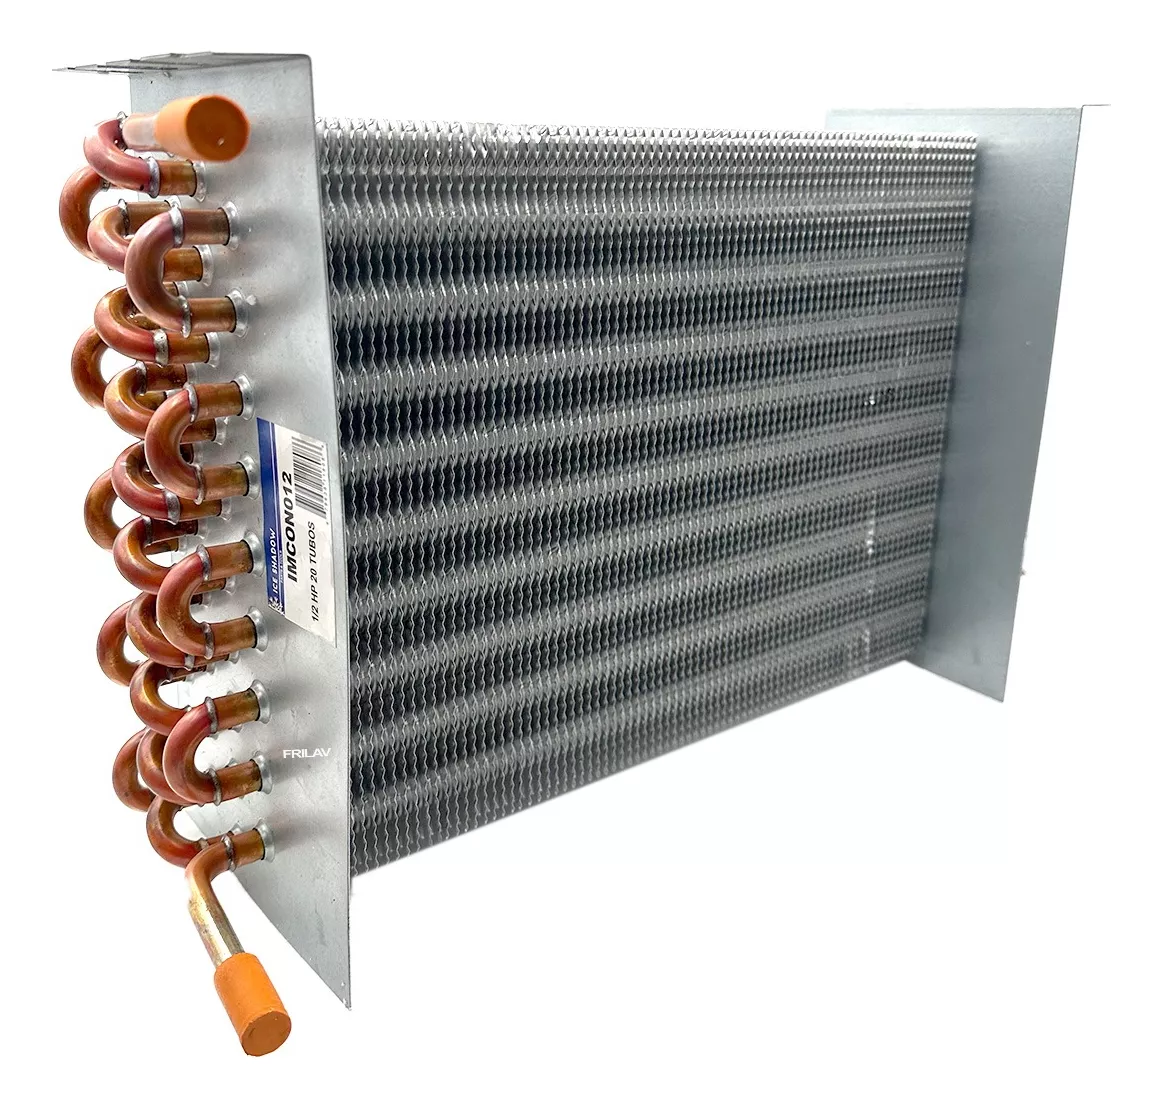
\includegraphics[width=0.45\linewidth]{figures/condensador}
	\caption{Condensador ICE SHADOW elegida para el proyecto}
	Fuente: Tomado de (\citeauthor{ml2024}, 2024).
	\label{fig:condensador}
\end{figure}

 
 
 
  \subsection{Comparación de Unidades Evaporadoras}
 
El análisis a continuación presenta las características y ventajas de los evaporadores de las marcas MABE y BOHN, comparando tres opciones disponibles para la refrigeración en la UMF40. La elección del evaporador adecuado dependerá de varios factores clave, como la capacidad de evaporación, la eficiencia energética, la facilidad de mantenimiento y la compatibilidad con la unidad condensadora seleccionada. Además, se evaluará el costo total de propiedad y la durabilidad de cada opción para asegurar un funcionamiento óptimo en condiciones de operación constantes. La selección final buscará equilibrar el rendimiento térmico y la eficiencia económica, asegurando una solución integral que cumpla con los requisitos técnicos y presupuestarios establecidos para la instalación  
 
 \begin{table}[H]
 	\caption{Comparación de unidades evaporadoras de Perfil BAJO}
 	Fuente: Elaboración propia, basado de \cite{bohn2024}.
 	\centering
 	\scalebox{0.7}{ 
 \begin{tabular}{@{}ccllcc@{}}
 	\toprule
 	\textbf{Opción} & \textbf{Proveedor/Marca} & \multicolumn{1}{c}{\textbf{Ventajas}}                                                                                       & \multicolumn{1}{c}{\textbf{Desventajas}}                                                                                                      & \textbf{Costo} & \multicolumn{1}{l}{\textbf{Elección}}       \\ \midrule
 	IEM MABE        & MABE                     & \begin{tabular}[c]{@{}l@{}}- Diseñado para \\   equipos pequeños\\ - Adecuada al equipo\\ - Proveedor Mexicano\end{tabular} & \begin{tabular}[c]{@{}l@{}}- Al ser de gama\\  baja su tiempo \\  de vida es menor.\end{tabular}                                              & \$40.00  USD       & \textcolor[HTML]{34ff34}{ \checkmark}       \\ \cmidrule(lr){3-4}
 	Reach IN (TA)   & BOHN                     & \begin{tabular}[c]{@{}l@{}}- Equipo completo \\ - Diseño compacto\\ - Vendido por EU\end{tabular}                           & \begin{tabular}[c]{@{}l@{}}- El equipo viene\\ armado y no es\\ conveniente comprarlo\\ porque no se usarán toda\\ su capacidad.\end{tabular} & \$1,750.00  USD    & \textbf{\textcolor[HTML]{fd6864}{\text{x}}} \\ \cmidrule(lr){3-4}
 	Reach IN (TL)   & BOHN                     & \begin{tabular}[c]{@{}l@{}}- Gabinete de aluminio\\ - Diseño compacto\\ - Vendido por EU\end{tabular}                       & \begin{tabular}[c]{@{}l@{}}- El equipo está diseñado\\ para cámaras de al menos\\ 2m de alto.\end{tabular}                                    & \$7,750.00  USD    & \textbf{\textcolor[HTML]{fd6864}{\text{x}}} \\ \bottomrule
 \end{tabular}
 	}
 \end{table}
 
 \subsubsection{Análisis de las Opciones}
 Cada una de las opciones presenta características particulares que pueden ser relevantes dependiendo de las necesidades específicas del proyecto en la UMF40. Es fundamental evaluar, no solo el costo, sino también la eficiencia operativa, la facilidad de mantenimiento y la capacidad de enfriamiento de cada unidad.
 
 \begin{itemize}
 	\item \textbf{IEM MABE} (1/8 HP): Esta opción se ajusta perfectamente a la carga térmica necesaria para la conservación de la insulina en la UMF40. Destaca por su bajo costo, facilidad de mantenimiento y su origen local, lo que facilita el acceso a repuestos y soporte. Sin embargo, su vida útil es más corta debido a ser una opción de gama baja, lo cual debe ser considerado en términos de costos operativos a largo plazo.
 	\item \textbf{Reach IN (TA)} (1/4 HP): A pesar de ser un equipo de alta calidad con diseño compacto y eficiencia energética, no cumple con los requerimientos de carga térmica para este proyecto. Además, su costo es elevado en comparación con el beneficio que aporta, lo que la hace menos atractiva para este tipo de aplicaciones específicas.
 	\item \textbf{Reach IN (TL)} (1/4 HP): Aunque su diseño es robusto y adecuado para espacios más grandes, no es compatible con los requisitos de tamaño de la cámara en la UMF40. El costo elevado y el diseño no adecuado para cámaras más pequeñas hacen que esta opción sea menos conveniente para este proyecto.
 \end{itemize}
 
 \subsubsection{Preferencia y Elección}
 La selección final se ha basado en un análisis exhaustivo de las opciones disponibles, considerando los requerimientos específicos del proyecto, el presupuesto disponible, y los beneficios a largo plazo. Tras evaluar la carga térmica necesaria, la eficiencia de los equipos, y los costos operativos, se determinó que la opción \textbf{IEM MABE} (1/8 HP) es la más adecuada.
 
 Esta opción no solo cumple con la carga térmica mínima requerida, sino que también ofrece un excelente balance entre costo y eficiencia operativa. Aunque su vida útil es más corta, su bajo costo inicial y su fácil mantenimiento la convierten en una opción sostenible para la cámara de refrigeración en la UMF40.
 
 El costo total de la opción \textbf{IEM MABE} es adecuado dentro del presupuesto asignado, lo que hace de esta elección una solución económica y efectiva para este proyecto. A nivel técnico, cumple con todos los requisitos de capacidad de enfriamiento y estabilidad térmica necesaria para el almacenamiento de insulina.
 
 En resumen, la opción \textbf{IEM MABE} (1/8 HP) ofrece el mejor equilibrio entre rendimiento, costo y facilidad de mantenimiento, lo que la convierte en la elección más adecuada para este proyecto de refrigeración médica.
 
 
 \begin{figure}[H]
 	\centering
 	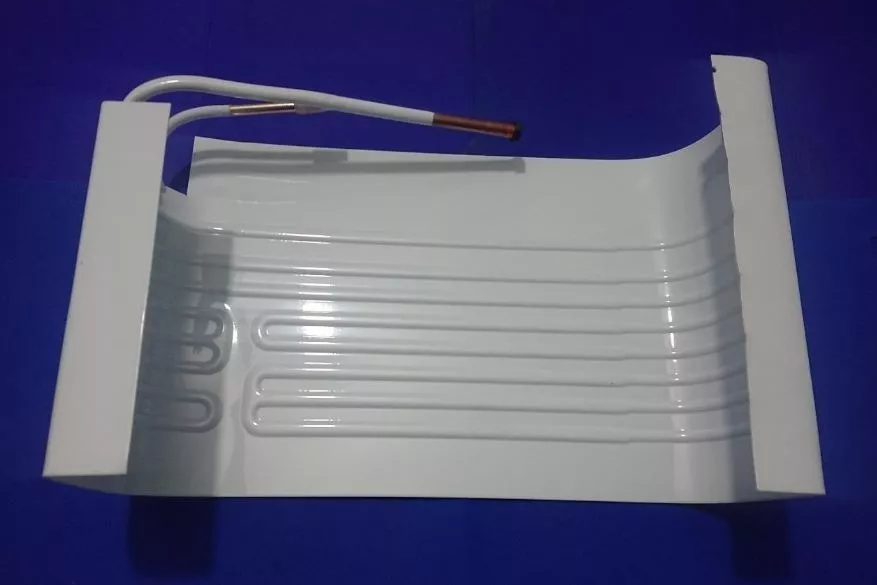
\includegraphics[width=0.6\linewidth]{figures/evaporador}
	\caption{Evaporador IEM MABE elegida para el proyecto}
	Fuente: Tomado de \cite{mabe2024}
 	\label{fig:evaporador}
 \end{figure}
 
  
 \subsection{Comparación de Unidades de motores eléctricos}
 
El análisis a continuación presenta las características y ventajas de los motores eléctricos para el sistema eléctrico del equipo, comparando tres opciones disponibles para su integración en la unidad de refrigeración de la UMF40 de Azcapotzalco.


 \begin{table}[H]
	\caption{Comparación de unidades motores eléctricos de potencia baja}
	Fuente: Elaboración propia, basado de \cite{ml2024}.
	\centering
	\scalebox{0.7}{ 
 \begin{tabular}{@{}ccllcc@{}}
 	\toprule
 	\textbf{Opción}                                                           & \textbf{Proveedor/Marca} & \multicolumn{1}{c}{\textbf{Ventajas}}                                                                                                                                                                           & \multicolumn{1}{c}{\textbf{Desventajas}}                                                                                                         & \textbf{Costo} & \multicolumn{1}{l}{\textbf{Elección}}          \\ \midrule
 	\begin{tabular}[c]{@{}c@{}}AP APPLI PARTS\\ APFM-51E \\ 120V\end{tabular} & Ap Appli Parts           & \begin{tabular}[c]{@{}l@{}}- La etapa de potencia\\ del equipo es similar \\ a la calculada\\ - Cuenta con protección \\ a fallas eléctricas.\\ - Es compatible con el \\ condensador y evaporador\end{tabular} & \begin{tabular}[c]{@{}l@{}}- Es genérico y debe \\ ser reemplazado en \\ el mantenimiento,\\ según las observaciones\\ del técnico.\end{tabular} & \$40.00 USD    & \textbf{\textcolor[HTML]{34ff34}{ \checkmark}} \\ \cmidrule(lr){3-4}
 	K50P-1125-001                                                             & DANFOS                   & \begin{tabular}[c]{@{}l@{}}- Precio menor\\ - Sistema más compacto\\ - Para equipos pequeños\end{tabular}                                                                                                       & \begin{tabular}[c]{@{}l@{}}- El sistema es sencillo\\ y no soportará cortos\\ circuitos\end{tabular}                                             & \$20.00 USD    & \textbf{\textcolor[HTML]{fd6864}{\text{x}}}    \\ \cmidrule(lr){3-4}
 	GenèricoRefri                                                             & Universal                & \begin{tabular}[c]{@{}l@{}}- Diseñado para sistemas pequeños\\ - Tamaño compacto\end{tabular}                                                                                                                   & \begin{tabular}[c]{@{}l@{}}- Motor genérico no \\ apto para el tiempo de \\ funcionamiento del equipo\\ médico.\end{tabular}                     & \$15.00 USD        & \textbf{\textcolor[HTML]{fd6864}{\text{x}}}    \\ \bottomrule
 \end{tabular}
	}
\end{table}


  
\subsubsection{Análisis de las Opciones}
Cada una de las opciones presenta ventajas y desventajas particulares que pueden ser relevantes dependiendo de las necesidades específicas de la cámara de refrigeración en la UMF40. A continuación, se justifica la elección del motor **AP APPLI PARTS APFM-51E 120V**:

\begin{itemize}
	\item \textbf{AP APPLI PARTS APFM-51E 120V}: Esta opción ha sido seleccionada debido a su adecuada compatibilidad con los componentes del sistema de refrigeración (condensador y evaporador). Además, su etapa de potencia es similar a la carga calculada para el proyecto, lo que garantiza un funcionamiento eficiente. Su protección a fallas eléctricas es una ventaja importante para mantener la seguridad del sistema. Aunque el motor es genérico y requiere reemplazo durante el mantenimiento, su costo accesible y su fiabilidad lo hacen ideal para este tipo de aplicación, donde la duración del equipo y los costos operativos son factores clave. 
	\item \textbf{K50P-1125-001 (DANFOS)}: Aunque tiene un costo relativamente bajo y es más compacto, esta opción presenta limitaciones en cuanto a su capacidad para soportar cortocircuitos. Además, la incompatibilidad con los requerimientos técnicos de la carga térmica hace que esta opción no sea adecuada para este proyecto.
	\item \textbf{GenèricoRefri (Universal)}: Aunque diseñado para equipos pequeños, este motor no es adecuado para los tiempos de funcionamiento de un equipo médico. Su vida útil limitada y las deficiencias en el rendimiento térmico lo hacen inapropiado para garantizar la eficiencia y seguridad en la conservación de insulina.
\end{itemize}

\subsubsection{Preferencia y Elección}
La opción seleccionada es el motor **AP APPLI PARTS APFM-51E 120V** debido a su fiabilidad, su compatibilidad con los componentes de refrigeración y su costo razonable. A pesar de ser un motor genérico, su protección contra fallas eléctricas y su adecuado rendimiento térmico lo convierten en la mejor opción para satisfacer los requisitos del sistema de refrigeración en la UMF40. Su bajo costo de adquisición y los beneficios a largo plazo en términos de mantenimiento hacen que esta opción sea la más adecuada para este proyecto.
  
 
  
  \begin{figure}[H]
  	\centering
  	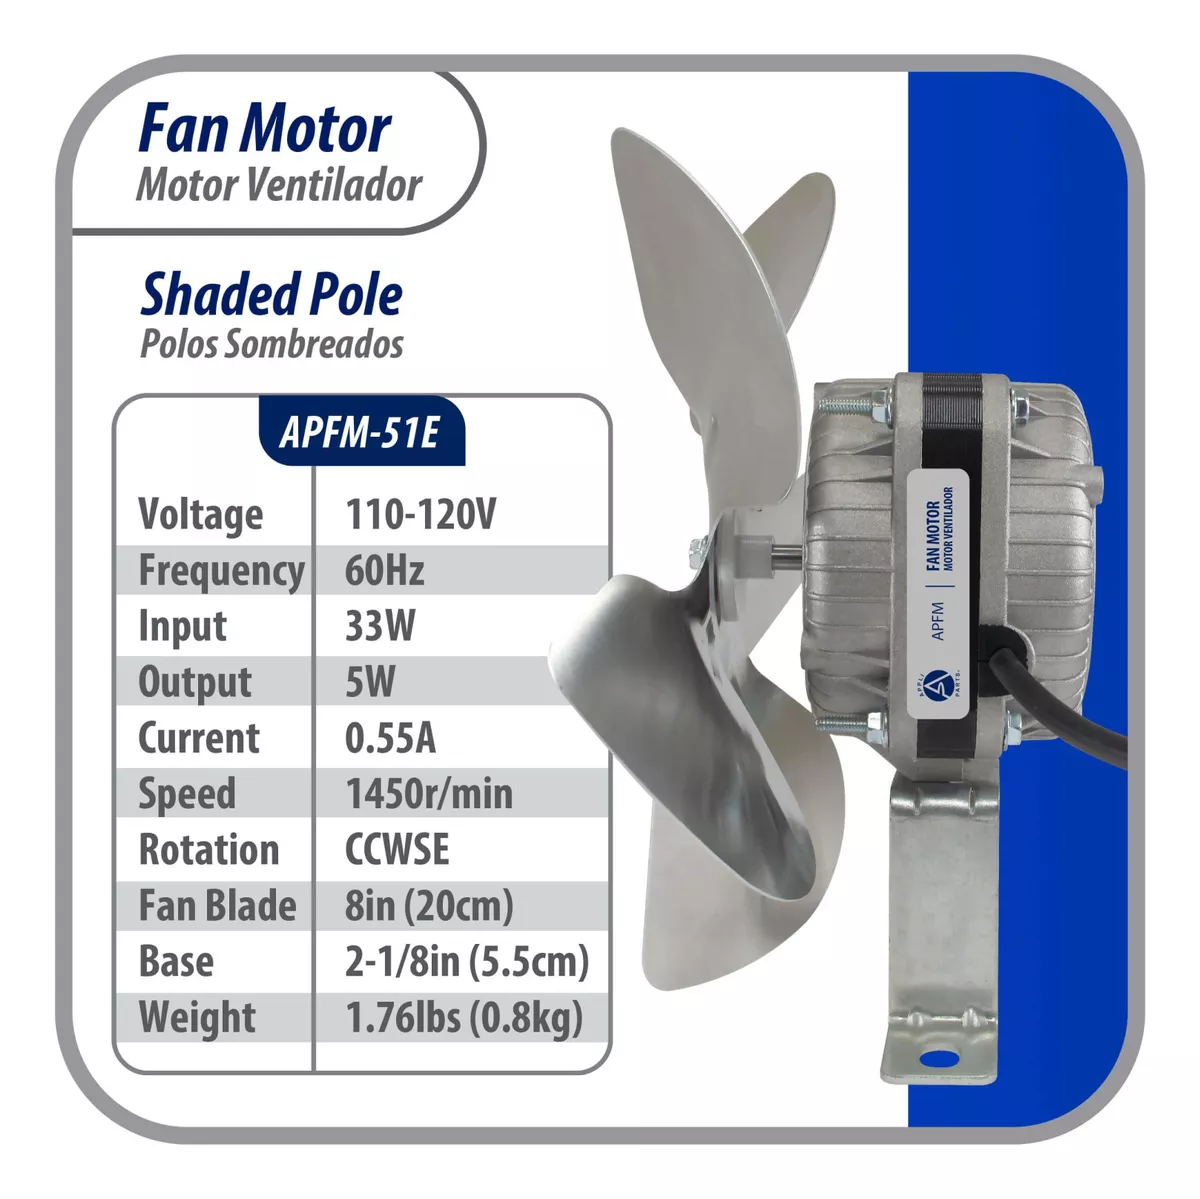
\includegraphics[width=0.5\linewidth]{figures/motorelectrico}
 	\caption{Motor eléctrico seleccionado para el proyecto}
Fuente: Tomado de (\citeauthor{ml2024}, 2024).
  	\label{fig:motorelectrico}
  \end{figure}
  
  
  \subsection{Selección del Aislante Térmico: Espuma de Poliuretano}
  
  El aislamiento térmico adecuado es esencial para cualquier sistema de refrigeración, especialmente en una cámara de refrigeración destinada a la conservación de productos perecederos como la insulina. Para reducir la transferencia de calor entre el interior y el exterior de la cámara, se seleccionó la espuma de poliuretano como el material aislante principal. Este material fue elegido debido a su excelente capacidad de aislamiento térmico, que permite alcanzar el espesor necesario para mantener condiciones de temperatura óptimas dentro de la cámara.
  
  El poliuretano es un material que ofrece una conductividad térmica muy baja, lo que lo convierte en un excelente aislante. Además, su ligereza es una característica clave, ya que permite mantener el peso total del sistema de refrigeración dentro de límites razonables, lo que optimiza el consumo de energía y facilita el transporte de la unidad refrigerada sin exceder la carga útil. La resistencia a la humedad y a la compresión del poliuretano garantiza que el material conserve sus propiedades a lo largo del tiempo, lo que prolonga la vida útil del sistema y asegura un rendimiento constante bajo diversas condiciones ambientales.
  
  El volumen total que se desea llenar con espuma de poliuretano es aproximadamente $2.5 ft^3$. Este volumen se calcula para cubrir las necesidades térmicas de aislamiento de la cámara, asegurando una eficiencia máxima en la conservación de la temperatura. De acuerdo con las especificaciones del producto seleccionado, el costo de un kit de espuma expansiva de poliuretano de 750 ml es de aproximadamente  {\$250.00 MXN }. El costo total estimado para el volumen requerido de poliuretano es de {\$1,250.00 MXN} \cite{poliuretanohomedepot}.
  
  El uso de poliuretano como material aislante no solo asegura el cumplimiento de los estándares térmicos necesarios para el transporte seguro de productos sensibles como la insulina, sino que también contribuye a la eficiencia energética y la durabilidad del sistema de refrigeración, lo que lo convierte en una opción ideal para este tipo de aplicaciones.
  
 
\subsection{Resumen costos indirectos}
A continuación, se ofrece una tabla resumen (\ref{tabla:costosdirectos}	) de los costos directos del proyecto.
\begin{table}[H]
	\caption{Tabla resumen de los costos directos del proyecto. (Elaboración propia)}
	\label{tabla:costosdirectos}
		\scalebox{0.8}{ 
	\begin{tabular}{@{}clclcc@{}}
		\toprule
		\textbf{\begin{tabular}[c]{@{}c@{}}Num \\ Unidades\end{tabular}} & \multicolumn{1}{c}{\textbf{Unidad}}       & \textbf{Descripción}                                                                   & \multicolumn{1}{c}{\textbf{Proveedor}}                                                   & \textbf{\begin{tabular}[c]{@{}c@{}}Precio \\ Unitario (MXN)\end{tabular}} & \textbf{\begin{tabular}[c]{@{}c@{}}Precio\\ Total (MXN)\end{tabular}} \\ \midrule
		1                                                                & \multicolumn{1}{c}{Condensador}           & \begin{tabular}[c]{@{}c@{}}Condensador de BAJA,\\ marca ICE SHADOW 1/8 HP\end{tabular} & \multicolumn{1}{c}{\begin{tabular}[c]{@{}c@{}}Mercado Libre\\ o ICE SHADOW\end{tabular}} & \textdollar{1,812.03}                                                           & \textdollar{1,812.03}                                                             \\
		1                                                                & \multicolumn{1}{c}{Evaporador}            & \begin{tabular}[c]{@{}c@{}}Evaporador de BAJA,\\ marca: Iem MABE\end{tabular}          & \multicolumn{1}{c}{MABE}                                                                 & \textdollar{805.35}                                                             & \textdollar{805.35}                                                               \\
		1                                                                & Motor eléctrico                           & \begin{tabular}[c]{@{}c@{}}Motor APFM-51E 120V,\\ Marca: APPLI PARTS\end{tabular}      & APPLI PARTS                                                                              & \textdollar{805.35}                                                             & \textdollar{805.35}                                                               \\
		3                                                                & Poliuretano                               & \begin{tabular}[c]{@{}c@{}}Poliuretano expandido\\  universal\end{tabular}             & HOME DEPOT                                                                               & \textdollar{254.00}                                                             & \textdollar{762.00}                                                               \\
		1                                                                & \multicolumn{1}{c}{Instalación de equipo} & \begin{tabular}[c]{@{}c@{}}Instalación de equipo de\\ refrigeración\end{tabular}       & \multicolumn{1}{c}{Contrato}                                                             & \textdollar{10,250.00}                                                           & \textdollar{10,250.00}                                                            \\ \cmidrule(r){1-4}
		\multicolumn{1}{l}{}                                             &                                           & \multicolumn{1}{l}{}                                                                   &                                                                                          & \multicolumn{1}{l}{IVA 16\%}                                                   & \textdollar{2,309.56}                                                             \\
		\multicolumn{1}{l}{}                                             &                                           & \multicolumn{1}{l}{}                                                                   &                                                                                          & \multicolumn{1}{l}{Importe Final}                                             & \textdollar{12,744.29}                                                            \\  \bottomrule
	\end{tabular}
}
\end{table}
  
  
\section{Costos Indirectos}

Los costos indirectos son aquellos gastos que no están directamente asociados con la producción de un bien específico o la prestación de un servicio en particular, pero que son necesarios para el funcionamiento general de un proyecto. En el caso de la instalación de una cámara de refrigeración para la conservación de insulina, estos costos incluyen el mantenimiento de los equipos, gastos administrativos, alquiler de instalaciones, seguros, servicios públicos y la depreciación de los activos involucrados.

En proyectos de infraestructura como la instalación de sistemas de refrigeración, los costos indirectos pueden representar hasta un 30\% del presupuesto total del proyecto. La correcta estimación de estos costos es esencial por varias razones:

\begin{itemize}
	\item Son fundamentales para calcular el presupuesto total y garantizar que todos los aspectos operativos estén cubiertos.
	\item Permiten tomar decisiones informadas sobre la asignación de recursos, la planificación financiera y las estrategias de mitigación de riesgos.
	\item Facilitan una evaluación precisa de la rentabilidad del proyecto, ayudando a determinar su viabilidad.
\end{itemize}

\subsubsection{Costos de Ingeniería}

El costo de ingeniería es un componente clave al evaluar proyectos de instalación de sistemas complejos, como las cámaras de refrigeración para la conservación de insulina, donde la precisión y eficiencia son cruciales. Este costo involucra los recursos necesarios para el diseño, planificación e implementación del proyecto, incluyendo mano de obra, materiales y tiempo invertido.

De acuerdo con datos de \textit{Data México} y la figura \ref{fig:mecanicos}, el salario promedio mensual de los ingenieros mecánicos en México, durante el segundo trimestre de 2024, es de \$8,830 MXN. Este monto puede variar dependiendo de la región y el sector, ya que los mejores salarios para ingenieros mecánicos se encuentran en estados como Durango (\$42,300 MXN) y Tlaxcala (\$32,000 MXN) \cite{salarioingeniero}. 

Para calcular el costo de ingeniería de un proyecto como el de instalación de una cámara de refrigeración, se toma en cuenta el salario promedio de un ingeniero mecánico y el tiempo estimado para llevar a cabo todas las etapas del proyecto. Por ejemplo, si un ingeniero recién egresado gana alrededor de \$8,830 MXN al mes y dedica aproximadamente 3 meses a la planificación y ejecución de la instalación del sistema de refrigeración, el costo de ingeniería total podría ascender a más de \$26,000 MXN, dependiendo de la complejidad y duración del proyecto.

La correcta estimación de estos costos es crucial para asegurar que el proyecto se ejecute dentro de los límites financieros establecidos, maximizando la eficiencia y evitando desviaciones presupuestarias. La planificación adecuada y la asignación de recursos también garantizarán que el sistema de refrigeración para la conservación de insulina cumpla con los estándares de calidad y seguridad necesarios.
 
 
  
  \begin{figure}[H]
  	\centering
  	\caption{Costos por el Ingenieroo o Técnico}
  	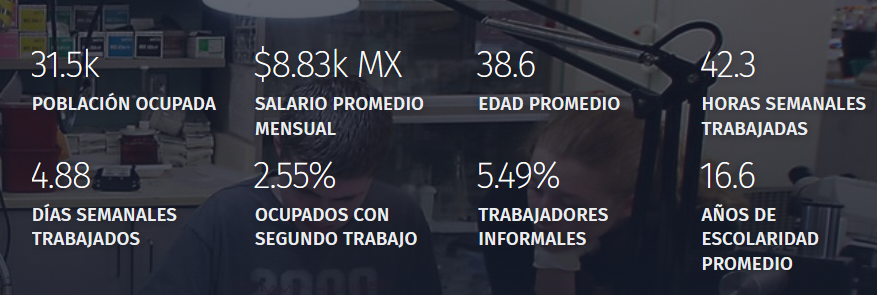
\includegraphics[width=0.6\linewidth]{figures/mecanicos}
  	\caption{Insights y KPI del perfil de Ingenieros Mecánicos en México}
  	Fuente: \cite{salarioingeniero}
  	\label{fig:mecanicos}
  \end{figure}
  
  En la figura \ref{fig:mecanicos} se puede observar el ingreso mensual promedio de un ingeniero mecánico recién egresado en 2024. Para poder obtener el sueldo por hora se hacen las operaciones
  necesarias.
  
  Salario promedio mensual = \$8,300.00 MXN\\
  Horas semanales trabajadas = 42.3 h\\
  Semanas que tienes un mes= 4\\
  Salario promedio por hora =  \$49.06 MXN\\
  
  Tomando en cuenta estos datos se calcula el tiempo total que se le dedicó al proyecto y el costo del mismo tiempo (Tabla \ref{tabla:costopersonal})
  
  
 \begin{table}[H]
 	\centering
 	\caption{ Costos del personal}
 	\label{tabla:costopersonal}
\begin{tabular}{@{}cccccl@{}}
	\toprule
	\multicolumn{6}{c}{Tiempo invertido en el proyecto}                                \\ \midrule
	Horas/día & Horas/semana & Horas/mes & Meses & Horas totales & Costo total         \\ \midrule
	2         & 10           & 40        & 7     & 280           & \$13,736.8 MXN. \\ \bottomrule
\end{tabular}
 \end{table}
  
  
  La tabla \ref{tabla:costopersonal} muestra el cálculo de las horas trabajadas por el autor de este trabajo durante el proyecto.Este costo considera el número de integrantes en el desarollo de todo el proyecto para cálculos posteriores, en este caso solo es una persona y asciende a un total de \$3,456,178.88 MXN.
  
  \subsubsection{Costos por adquisición}
  Los costos de adquisición representan una inversión esencial para garantizar la ejecución exitosa del proyecto, incluyendo todos los elementos necesarios para su desarrollo. Entre estos, se consideran materiales técnicos como componentes para la cámara de refrigeración (condensador, evaporador y motor), servicios contratados para la instalación y puesta en marcha, así como recursos administrativos como papelería y permisos. Además, se incluyen los costos asociados a herramientas tecnológicas, como equipo de cómputo y licencias de software especializadas, como ANSYS, utilizadas para las simulaciones térmicas y el diseño estructural. La Tabla \ref{tabla:costos-adquisicion} resume detalladamente estos costos, permitiendo visualizar su distribución y su impacto en el presupuesto global del proyecto.
  
  % Please add the following required packages to your document preamble:
  % \usepackage{booktabs}
  \begin{table}[H]
  	\centering
  	\caption{Costos de adquisición. (Elaboración propia)}
  	\label{tabla:costos-adquisicion}
  	\begin{tabular}{@{}llll@{}}
  		\toprule
  		\multicolumn{1}{c}{Concepto}                                                                             & \multicolumn{1}{c}{Cantidad} & \multicolumn{1}{c}{Precio por unidad} & \multicolumn{1}{c}{Costo total} \\ \midrule
  		Bolígrafos                                                                                               & 3 unidades                   & \$ 7.00 MXN                            & \$21.00 MXN                     \\
\  		Hojas                                                                                                    & 1 paquete                    & \$129.00MXN                            & \$129.00 MXN                    \\
  		Folders                                                                                                  & 5 unidades                   & \$5.00 MXN                             & \$25.00 MXN                     \\
  		Impresiones                                                                                              & 150 hojas                    & \$1.00 MXN                             & \$150.00 MXN                    \\
  		\begin{tabular}[c]{@{}l@{}}Libro Buenas prácticas\\ de refrigeración y aire\\ acondicionado\end{tabular} & 1 unidad                     & \$250.00 MXN                           & \$250.00 MXN                    \\
  		Libro Refrigeración                                                                                      & 1 unidad                     & \$700.00 MXN                           & \$700.00 MXN                    \\
  		Internet                                                                                                 & 7 meses                      & \$599.00 MXN                           & \$4193.00 MXN                   \\
  		Software(SolidWorks)                                                                                     & Licencia 1 año               & \$84,602.00 MXN                        & \$84,602.00 MXN                 \\
  		Laptops                                                                                                  & 1 equipos                    & \$22,000.00 MXN                        & \$22,000.00 MXN                 \\
  		Pasajes                                                                                                  & 20 vueltas                   & \$20.00                                & \$400.00 MXN                    \\
  		&                              & \multicolumn{1}{r}{\textbf{TOTAL}}             & \$112,470.00 MXN                \\ \bottomrule
  	\end{tabular}
  \end{table}
  
  El total de los costos de adquisición que se obtiene a lo largo del proyecto es de  \$112,470.00 MXN  los cuales forman parte de los gastos indirectos del proyecto
  
  \subsubsection{Costo de desarrollo del proyecto}
  
  Los costos asociados al desarrollo del proyecto comprenden los gastos necesarios para garantizar su planificación, ejecución y conclusión exitosa. Este apartado incluye elementos como la mano de obra técnica, los materiales específicos para la construcción y montaje, la adquisición de tecnología, servicios de consultoría y capacitación especializada. En el caso particular de este proyecto, se realizaron consultorías técnicas enfocadas en la selección y dimensionamiento de equipos de refrigeración, así como en la integración de los accesorios del sistema eléctrico. Estas asesorías fueron fundamentales para asegurar que los componentes seleccionados cumplieran con las especificaciones técnicas requeridas, optimizando tanto el rendimiento del sistema como su costo. La Tabla \ref{tabla:costos-desarrollo} detalla la relación entre las horas invertidas en asesoramiento y el costo correspondiente, tomando como referencia el salario promedio de un ingeniero mecánico especializado en refrigeración.
  
  
  
  
  % Please add the following required packages to your document preamble:
  % \usepackage{booktabs}
  \begin{table}[]
  	\centering
  	\caption{Tabla de costos del desarrollo del proyecto}
  	\label{tabla:costos-desarrollo}
  	\begin{tabular}{@{}ccccc@{}}
  		\toprule
  		Horas/mes & Num. meses & Total de horas & Salario/hora & Total         \\ \midrule
  		2         & 7          & 14             & \$49.06 MXN  & \$ 686.84 MXN \\ \bottomrule
  	\end{tabular}
  \end{table}
  
  \subsection{Costo de la Protección Económica del Proyecto}
  La protección económica de un proyecto es un elemento clave para salvaguardar sus finanzas y garantizar su viabilidad a largo plazo. Desde la concepción hasta la ejecución, los proyectos están expuestos a diversos factores internos y externos que pueden afectar su estabilidad financiera. Por ello, es fundamental considerar un porcentaje de "protección financiera" que permita mitigar posibles riesgos. Este porcentaje suele oscilar entre el 25\% y el 42\% del costo subtotal, dependiendo de la naturaleza y los requerimientos específicos del proyecto.
  
  Para este proyecto en particular, se ha determinado un porcentaje de protección económica del 30\%, el cual se calcula sumando los costos directos e indirectos asociados. El costo directo del proyecto asciende a \$12,744.2 MXN, mientras que el costo indirecto es de \$126,893.64 MXN. Al sumar ambos conceptos, se obtiene un subtotal de \$139,637.84 MXN, sobre el cual se aplica el porcentaje de protección económica.
  
  El monto destinado a la protección económica, equivalente al 30\% del subtotal, asciende a \$41,891.35 MXN. Este fondo adicional asegura que el proyecto disponga de los recursos necesarios para enfrentar contingencias financieras, garantizando su correcta ejecución y sostenibilidad a lo largo del tiempo (Tabla \ref{tabla:5costoprote}).
  
  \begin{table}[H]
  	\centering
  	\caption{Costo de la protección económica del proyecto.}
  	\label{tabla:5costoprote}
  	\begin{tabular}{@{}cc@{}}
  		\toprule
  		Concepto                                       & Costo (MXN)                       \\ \midrule
  		Subcosto                                       & \$ 139,637.84                     \\
  		\multicolumn{1}{l}{Protección económica (30\%)} & \multicolumn{1}{l}{\$ 181,529.19} \\ \bottomrule
  	\end{tabular}
  \end{table}
  
  
  
  \subsection{Costo Total del Proyecto}
  El costo total del proyecto se calcula sumando los costos directos e indirectos, obtenidos previamente como sub-costo, y el monto destinado a la protección económica. Este cálculo asegura que se incluyan todos los factores necesarios para la correcta ejecución y sostenibilidad del proyecto.
  
  \begin{table}[H]
  	\caption{Costo total del proyecto}
  	{Fuente: Elaboración propia (2024)}\\
  	\centering
  	\label{tabla:costo-total}
  	\begin{tabular}{lr}
\toprule
  		 {Concepto}             &  {Cantidad (MXN)} \\ \midrule
  		Sub-costo                     & \$139,637.84            \\  
  		Protección económica (30\%)   & \$41,891.35             \\  
  		 {Costo total}          &  {\$181,529.19}   \\ \bottomrule
  	\end{tabular}
  \end{table}
  
  \subsection{Costo de Venta del Proyecto}
  El costo de venta del proyecto se determina considerando varios factores, entre ellos el costo de producción, el margen de beneficio, el análisis de mercado, y las posibles contingencias. Para este proyecto, el margen de utilidad se ha definido en un 34\% sobre el costo total calculado. Este porcentaje asegura que el proyecto sea viable financieramente y permita un retorno de inversión adecuado.
  
  \begin{table}[H]
  	\caption{Costo de venta del proyecto}
  	{Fuente: Elaboración propia (2024)}\\
  	\centering
  	\label{tabla:costo-venta}
  	\begin{tabular}{lr}
  		\toprule
  		{Concepto}             & {Cantidad (MXN)} \\ \midrule
  		Costo total                   & \$181,529.19            \\  
  		Porcentaje de venta (34\%)    & \$61,719.93             \\  
  		 {Costo de venta}       &  {\$243,249.12}   \\  \bottomrule
  	\end{tabular}
  	
  \end{table}
  
  Como resultado, el costo de venta del proyecto asciende a un total de \$243,249.12 MXN. Este monto considera todos los factores relevantes, asegurando la viabilidad del proyecto sin pérdidas y garantizando un margen de beneficio sostenible para su implementación y comercialización.
  
  
  
  \section{Conclusión}
  
  
  El desarrollo de este proyecto representa un avance significativo en la mejora de las condiciones de conservación de medicamentos críticos, como la insulina, en un entorno urbano complejo como la Ciudad de México. A lo largo del trabajo, se abordaron múltiples aspectos esenciales para garantizar la viabilidad técnica y económica de la cámara de refrigeración diseñada específicamente para la Unidad Médica Familiar (UMF) 40.
  
  El análisis comenzó con la identificación de las necesidades particulares del entorno, como las fluctuaciones de temperatura y la altitud de 2,240 m sobre el nivel del mar, las cuales imponen restricciones únicas sobre el diseño y operación de los sistemas de refrigeración. A partir de estas condiciones, se realizó un cálculo detallado de la carga térmica, el cual consideró factores como la temperatura de almacenamiento requerida de 2°C a 8°C y las propiedades de los materiales seleccionados para el aislamiento térmico, como el poliuretano expandido. Estos cálculos fueron la base para la selección precisa de componentes clave, como el condensador, evaporador y motor eléctrico, asegurando que cada uno cumpla con los requisitos de eficiencia energética y capacidad operativa.
  
  La selección del equipo no solo estuvo orientada a cumplir con las especificaciones técnicas, sino también a garantizar la sostenibilidad financiera del proyecto. Se evaluaron cuidadosamente los costos directos, indirectos y el porcentaje de protección económica, asegurando una gestión financiera robusta. El costo total del proyecto se calculó de manera integral, lo que permite no solo su implementación inmediata, sino también su viabilidad a largo plazo, con un enfoque en la reducción de costos operativos y el cumplimiento de normativas médicas internacionales.
  
  Desde un punto de vista técnico, la cámara de refrigeración integra principios modernos de ingeniería térmica y ciencia de materiales. La compatibilidad entre los componentes seleccionados, como el evaporador de bajo perfil de MABE y el motor eléctrico AP APPLI PARTS, optimiza el rendimiento del sistema al mantener temperaturas constantes de manera eficiente y confiable. 
  
  La implementación de esta solución no solo asegura la conservación de insulina en condiciones óptimas, sino que también establece un precedente para futuros proyectos en el ámbito médico. La tecnología aplicada en este proyecto puede ser adaptada a otras necesidades críticas de almacenamiento, contribuyendo al fortalecimiento del sistema de salud mediante la reducción de pérdidas de medicamentos y la mejora en la calidad de atención a los pacientes.
  
 Finalmente, este proyecto logra un balance integral entre viabilidad técnica, sostenibilidad financiera y cumplimiento de los estándares médicos más exigentes. La cámara de refrigeración diseñada para la UMF 40 no solo resuelve un problema específico, sino que también ofrece una solución replicable y escalable, posicionándose como un ejemplo de cómo la ingeniería y la tecnología pueden contribuir significativamente al bienestar social.
  
  
  \section{Recomendaciones}
  Para garantizar el correcto funcionamiento, durabilidad y eficiencia de la cámara de refrigeración diseñada para la conservación de insulina, se proponen las siguientes recomendaciones:
  
  \begin{enumerate}
  	\item \textbf{Mantenimiento regular:}
  	\begin{itemize}
  		\item Realizar inspecciones periódicas para verificar el estado de todos los componentes, incluyendo el sistema de refrigeración, el aislamiento y las juntas de las puertas.
  		\item Limpiar los componentes regularmente para evitar la acumulación de polvo y suciedad, que pueden reducir la eficiencia del enfriamiento.
  		\item Programar revisiones profesionales con técnicos especializados para detectar y corregir cualquier problema potencial antes de que se convierta en un fallo mayor.
  	\end{itemize}
  	
  	\item \textbf{Control de temperatura:}
  	\begin{itemize}
  		\item Monitorear constantemente la temperatura interna de la cámara para asegurarse de que se mantenga dentro del rango deseado.
  		\item Verificar regularmente el funcionamiento de las alarmas de temperatura para asegurar una detección inmediata de anomalías.
  	\end{itemize}
  	
  	\item \textbf{Manejo adecuado:}
  	\begin{itemize}
  		\item No sobrecargar la cámara; asegúrese de no exceder la carga diseñada y permita suficiente espacio para la circulación del aire frío.
  		\item Distribuir los elementos de manera uniforme para evitar puntos calientes y garantizar una refrigeración homogénea.
  	\end{itemize}
  	
  	\item \textbf{Cuidados del sistema:}
  	\begin{itemize}
  		\item Inspeccionar las conexiones eléctricas y los cables para detectar desgaste o daños, asegurándose de que las conexiones estén seguras y libres de corrosión.
  	\end{itemize}
  	
  	\item \textbf{Sellos y puertas:}
  	\begin{itemize}
  		\item Revisar regularmente las juntas de las puertas para asegurarse de que no haya fugas de aire. Reemplazar cualquier junta dañada.
  		\item Asegurarse de cerrar correctamente las puertas y evitar abrirlas innecesariamente para mantener la temperatura interna.
  	\end{itemize}
  	
  	\item \textbf{Limpieza y desinfección:}
  	\begin{itemize}
  		\item Limpiar y desinfectar regularmente el interior de la cámara para evitar la acumulación de bacterias y moho. Usar productos de limpieza adecuados según las instrucciones del fabricante.
  	\end{itemize}
  	
  	\item \textbf{Ventilación:}
  	\begin{itemize}
  		\item Asegurarse de que el área alrededor de la cámara esté bien ventilada para evitar el sobrecalentamiento del motor y otros componentes.
  		\item Evitar bloquear las ventilas del sistema de refrigeración para mantener la eficiencia operativa.
  	\end{itemize}
  	
  	\item \textbf{Movilidad y transporte:}
  	\begin{itemize}
  		\item Mover la cámara con cuidado para evitar golpes y daños estructurales.
  	\end{itemize}
  	
  	\item \textbf{Almacenamiento adecuado:}
  	\begin{itemize}
  		\item Cuando no esté en uso, almacenar la cámara en un lugar seco, bien ventilado y protegido de la exposición directa al sol y temperaturas extremas.
  		\item Antes de almacenarla por períodos prolongados, desconectar, limpiar y secar completamente la cámara para evitar la formación de moho y malos olores.
  	\end{itemize}
  	
  	\item \textbf{Capacitación del personal:}
  	\begin{itemize}
  		\item Asegurarse de que todo el personal que maneja la cámara esté capacitado adecuadamente en su uso y mantenimiento.
  		\item Proporcionar acceso al manual de usuario y asegurar que se sigan todas las recomendaciones del fabricante.
  	\end{itemize}
  \end{enumerate}
  
  
  